\section{Introduction}

A wide variety of problems in machine learning can be framed as probabilistic inference. In particular, latent variable models learn representations of data that capture salient characteristics of its underlying distribution, which can then be used for downstream tasks such as classification \cite{klingler2017efficient}. While traditional inference techniques can be slow or even computationally intractable, the advent of \textit{amortized  inference} allowed such methods to scale to large datasets, bringing about significant progress in generative modeling applications such as image and audio synthesis \cite{brock2018large,oord2016wavenet}, molecule generation \cite{segler2017generating}, and more.

However, as the problem domains we face become increasingly more complex and multimodal, a technical challenge arises: generative models trained using traditional inference techniques struggle to adapt to new data distributions, even when these new distributions may be \textit{closely related} to distributions seen during training. For example, variational autoencoders (VAEs) trained on the original image distributions have difficulty generalizing to small visual transformations such as
changing the position or quantity of objects in the scene. 
However, we would expect the true generative model, such as those of humans \cite{yildirim2014perception}, to be invariant to these slight modifications. Therefore, the question we aim to address is: 
how do we design an amortized inference algorithm that 
generalizes across 
%shares statistical strength between 
related distributions to learn \textit{transferable} representations? Such features would capture the salient characteristics necessary to allow for better generalization to related, but unseen distributions at test time.
% that are \textit{transferable} to a family of transformations, while also preserving the tractability of amortized inference? 

To address this question, we propose a \textit{doubly-amortized} inference procedure that amortizes computation across not only a set of query inputs, but also a \textit{set} of different, related target probabilistic models.
% , each of which capture a single data distribution. 
More precisely, we derive a new objective called the MetaELBO which serves as a variational lower bound across multiple distributions, while also incorporating a prior regularization term encouraging each generative model to match its respective data marginal.
We note that this inference model is not intended to be universal, but rather tailored to a specific family where each  probabilistic model is similar in structure. 
Inspired by meta-learning, we denote this "doubly-amortized" inference problem as \textit{meta-inference} and let a \textit{meta-distribution} refer to the distribution over probabilistic models. 

As an instantiation of our method, we introduce the MetaVAE, a VAE trained with the MetaELBO. 
% We showcase our approach in a variety of settings. 
Empirically, we first show three demonstrations to build intuition for meta-inference: 1) clustering, 2) compiled inference, and 3) learning sufficient statistics on exponential families. Then, we study image transformations (e.g. rotations, shearing) on MNIST digits where the MetaVAE learns representations that transfer to unseen transformations, outperforming baselines by 10-50\%. Finally, we showcase similar improvements of 10-35\% on real-world images (NORB).
% show a similar study with real world images (NORB) that finds improvements of 10-35\%. 
While the representations learned from other generative models quickly decay in quality under more severe transformations, those of the MetaVAE preserve relevant information about the image while abstracting away unnecessary differences induced by visual manipulation. 

\section{Meta-Amortized Variational Inference}
\label{sec:meta}

% \s{this section could use more intuition and motivation for why we are doing this. see comments below}

% As motivation, we build on the medical example presented in the previous section. 
% \cc{If you jump to this section you are confused as the medical motivation is split across a sub-heading. Maybe start this section with the previous half of the last paragraph?}
The variational autoencoder (VAE) is a popular model for many real-world domains: in medical diagnosis, for example, one can infer the identity of a disease ($z$) from observed symptoms ($x$). Given a set of symptoms from a population of patients, we can fit a VAE tailored to a disease, e.g. thoracic disease \cite{mao2018deep}.
But in practice, physicians often work with several patient populations that vary across a wide range of socioeconomic factors. For a new population, clinicians draw on prior experience from patients with similar symptoms, lowering their chances of misdiagnosis. 
We can similarly construct a generative model that captures this intuition. 
% Given many distributions of patients, we would like to share statistical strength between them to infer latent features that transfer to similar, but previously unseen populations.
Instead of training a VAE on a new population, which would be equivalent to the physician re-learning how to diagnose an illness, we aim to share statistical strength between different patient groups to infer latent features that transfer to similar, but previously unseen populations.
We formalize this idea into a new algorithm that we call \textit{meta-amortized inference}.

Recall a (singly)-amortized inference model for $p_\theta(x,z)$
\begin{equation}
\max_{\phi}\mathbf{E}_{p_{\textup{data}}(x)} \left[ \mathbf{E}_{f_\phi(x)} \log \frac{p_\theta(x,z)}{f_\phi(x)(z)} \right]
\end{equation}
% \s{this will be confusing because it doesn't look like the equation we showed before}
which approximates $p_\theta(z|x)$ for various choices of the observed variables, $x \sim p_{\textup{data}}(x)$. Recall from Section~\ref{sec:background} that $f_\phi: X \rightarrow \mathcal{Q}$ is a supervised regressor that maps observations to posterior distributions. Unlike Equation~\ref{eq:elbo}, we have written $q_\phi(z|x)$ in its alternate form, $f_\phi(x)(z)$.

We are now interested in not one but a set of models,
$\mathcal{J}_\mathcal{I} = \{p_{\theta_i}(x,z), i \in \mathcal{I}\}$ where $\mathcal{I}$ is a finite set of indices.  
% = \{p(z)p_{\theta_i}(x|z), i \in \mathcal{I}\}$  <-- whats the point of writing this
Crucially, (like the example above) we make a few simplifying assumptions. First, we assume that the random variables in each model have the same domains (e.g. $X,Z$), but the relationships between the random variables may be different.
% -- this is to ensure that the inference problem is tractable \kristy{is this true?}. 
Second, we assume that for each model, we care about the same inference query $p_{\theta_i}(z|x)$. Finally, we assume to have some knowledge of typical values of the observed variables for each model in $\mathcal{J}_\mathcal{I}$: formally, we desire a set $\mathcal{M}_\mathcal{I} = \{ p_{\textup{data}_i}, i \in \mathcal{I} \} \subseteq \mathcal{M}$ of marginal distributions over the observed variables. 
% \s{can we change notation to something more similar to the previous pdata?}
Here, $\mathcal{M}$ denotes the set of all possible marginal distributions over $X$. Let $p_{\mathcal{M}}: \mathcal{M}_\mathcal{I} \rightarrow [0,1]$ denote a distribution over $\mathcal{M}_\mathcal{I}$. For example, $p_{\mathcal{M}}$ may be uniform over a finite number of marginals. As $p_{\mathcal{M}}$ is a distribution over distributions, we refer to it as a \textit{meta-distribution}.

The naive approach to amortize over a set of models is:
\begin{equation}
\mathbf{E}_{p_{\textup{data}_i} \sim p_{\mathcal{M}}} \left[
\max_{\phi}\mathbf{E}_{p_{\textup{data}_i}} \left[ \mathbf{E}_{f_\phi(x)} \log \frac{p_{\theta_i}(x,z)}{f_\phi(x)(z)} \right] \right]
\end{equation}
where we separately fit an amortized inference model for each $p_{\theta_i}(x,z)$. However, this approach is prohibitively expensive as the size of $\mathcal{M}_{\mathcal{I}}$ increases, and training across models is decoupled.
% , as we cannot feasibly train too many inference networks in parallel. To remedy this issue, 
We instead propose to doubly-amortize the inference procedure as follows (we move the $\max$ out once more):
\begin{equation}
\max_{\phi} \mathbf{E}_{p_{\textup{data}_i} \sim p_{\mathcal{M}}} \left[
\mathbf{E}_{p_{\textup{data}_i}} \left[ \mathbf{E}_{g_\phi(p_{\textup{data}_i}, x)} \log \frac{p_{\theta_i}(x,z)}{g_\phi(p_{\textup{data}_i},x)(z)} \right] \right] 
\label{eqn:meta1_obj}
\end{equation}
where the original regressor $f_\phi(x)$ is replaced by a doubly-amortized regressor $g_\phi(p_{\textup{data}_i},x)$ that takes \textit{both} the marginal distribution $p_{\textup{data}_i}$ and an observation $x$ to return a posterior distribution. Formally, we call such a mapping, $g_\phi: \mathcal{M} \times X \rightarrow \mathcal{Q}$, a \textit{meta-inference model}. This doubly-amortized inference procedure must be robust across varying marginals and evidence, generalizing over $\mathcal{M}$: a large set of sufficiently similar, previously \textit{unseen} models. 

We note that the choice of $p_{\textup{data}_i}$ as input to $g_\phi$ is critical in practice. As with ELBO, a successful learning algorithm will learn generative models such as $p_{\theta_i}(x)$ or $p_{\theta_i}(x, z)$ that match $p_{\textup{data}_i}$.
But similar to recent progress in wake-sleep \cite{hinton1995wake,bornschein2014reweighted,le2018revisiting}, we found that using observations from the true marginal $p_{\textup{data}_i}$ led to significantly more stable training.
One may also consider alternate combinations of inputs for $p_{\textup{data}_i}$, which we leave as future work.

\paragraph{Meta-Amortized Variational Bayes and Learning}
In certain settings, we are given a set of generative models $\{p_{\theta_i^*}(x, z), i \in \mathcal{I} \}$, where each model $p_{\theta_i^*}(x, z)$ with known parameters  captures a marginal distribution, $p_i(x) \in \mathcal{M}_{\mathcal{I}}$. 
We can then immediately optimize Equation~\ref{eqn:meta1_obj} to obtain the optimal meta-inference model. 

But in many cases the generative models are not known ahead of time, and therefore we must jointly learn $\{\theta_i,  i \in \mathcal{I}\}$ along with the parameters of the meta-inference model, $\phi$. To do so, we consider the objective, 
% Obtaining such a set $\mathcal{J}_\mathcal{I} = \{p_{\theta_i}(x,z), i \in \mathcal{I}\}$ of similarly related generative models  is difficult. However, 
% Just as amortized variational inference works particularly well when learning the parameters of the generative model jointly with those of the amortized inference model, we can ``meta-learn" a \textit{set} of  generative models jointly with a \emph{single} doubly-amortized inference model.
%This is especially desirable for VAEs as given a new marginal distribution $p_i(x)$ and an observation $x$, we are able to make inferences directly for $x$ without having to learn a new generative model tailored to $p_i(x)$. 
% To meta-learn a VAE, we can jointly optimize the parameters of the meta-inference network $\phi$ and the parameters of each generative network $\theta_i$, $i \in \mathcal{I}$ according to this objective:
\begin{equation}
\max_{\phi} \mathbf{E}_{p_{\textup{data}_i} \sim p_\mathcal{M}} \left[ \max_{\theta_i}  
%\mathcal{L}(\phi, \theta, p_i, x) 
\mathcal{L}_{\phi, \theta_i}(p_{\textup{data}_i}) 
\right]
\label{eqn:meta2_obj}
\end{equation}
% \begin{equation}
% \max_{\phi} \mathbf{E}_{p_i \sim p_\mathcal{M}} \left[ \max_{\theta_i} \mathbf{E}_{x \sim p_i} \left[
% %\mathcal{L}(\phi, \theta, p_i, x) 
% \mathcal{L}_{\phi, \theta_i}(p_i) 
% \right] \right]
% \label{eqn:meta2_obj}
% \end{equation}
where the inner loss function is defined as:
\begin{equation*}
    \mathcal{L}_{\phi, \theta_i}(p_{\textup{data}_i}) = -\textup{KL}(p_{\textup{data}_i} g_\phi(p_{\textup{data}_i}, x), p(z)p_{\theta_i}(x|z))
    % \label{eqn:meta2_comp}
\end{equation*}
and $p_{\textup{data}_i} g_\phi(p_{\textup{data}_i}, x)$ denotes the distribution defined implicitly by first sampling $x \sim p_i(x)$, then sampling $z \sim g_\phi(p_{\textup{data}_i}, x)$. We refer to this lower bound as the MetaELBO, and a VAE trained with this objective as the MetaVAE. 

Lastly, we can rewrite the MetaELBO in a more interpretable form. Similar to $f_\phi(x)$, our regressor $g_\phi(p_{\textup{data}_i}, x)$ can be represented as a conditional distribution, denoted $q_\phi(z|p_{\textup{data}_i}, x) = g_\phi(p_{\textup{data}_i}, x)(z)$.
% \s{no big deal, but not swapping the order of x and Pd might avoid confusion}
Then,
%\mike{is this right}
\begin{align*}
    \mathcal{L}_{\phi, \theta}(p_{\textup{data}_i}) &= -\textup{KL}(p_{\textup{data}_i} \cdot q_\phi(z| p_{\textup{data}_i}, x),  p(z) \cdot p_{\theta_i}(x|z)) \\
    %&= -D_{KL}(q_\phi(x,z|p_i)||p_\theta_i(x,z)) \\
    &= -\textup{KL}(p_{\textup{data}_i}, p_{\theta_i}(x))  -\mathbf{E}_{x \sim p_{\textup{data}_i}}[\textup{KL}(q_\phi(z|p_{\textup{data}_i}, x), p_{\theta_i}(z|x))].
\end{align*}
This form has a penalty term for each distribution $p_{\textup{data}_i}$, encouraging the meta-amortized inference model to perform well across $p_{\textup{data}_i}$ sampled from the meta-distribution $p_{\mathcal{M}}$. We note that if $\mathcal{M} = \{p_{\textup{data}}\}$, then $g_\phi(p_{\textup{data}_i}, x) = f_\phi(x)$, and the MetaELBO is equivalent to ELBO. 

Interestingly, we find that the MetaVAE's learned representations transfer well to unseen downstream tasks at test time. We provide some intuition as to why this is the case. Samples from the corresponding marginal $p_{\textup{data}_i}$ help to lower the variance in the meta-inference network's inferred $z$'s for each query point $x$, regularizing the model's behavior to yield more robust representations.

\subsubsection{Representing the Meta-Distribution}
In Equation~\ref{eqn:meta2_obj}, it is not clear how to represent a distribution  $p_{\textup{data}_i}$ as input if we parameterize $g_\phi(p_{\textup{data}_i}, x)$ as a neural network. One of the main insights from this work is to represent the marginal distribution as a finite set of samples, 
\begin{equation}
    % p_i(x) \approx 
    \mathcal{D}_i = \{x_j \sim p_{\textup{data}_i} | j=1,...,N\}
\end{equation}
% \s{still doesn't type check, maybe you want sim instead of in?}
or a \textit{data set}. 
We can then use $\mathcal{D}_i$ to define an empirical analogue to $g_\phi(p_i, x)$, denoted as $\hat{g}_\phi:X^N \times X \rightarrow \mathcal{Q}$, which maps a data set with $N$ samples and an observation to a posterior. Then, there is an equivalent analogue of Equation~\ref{eqn:meta2_obj} where a marginal, $p_{\textup{data}_i}$ is replaced by a data set, $\mathcal{D}_i$. 

\begin{figure}
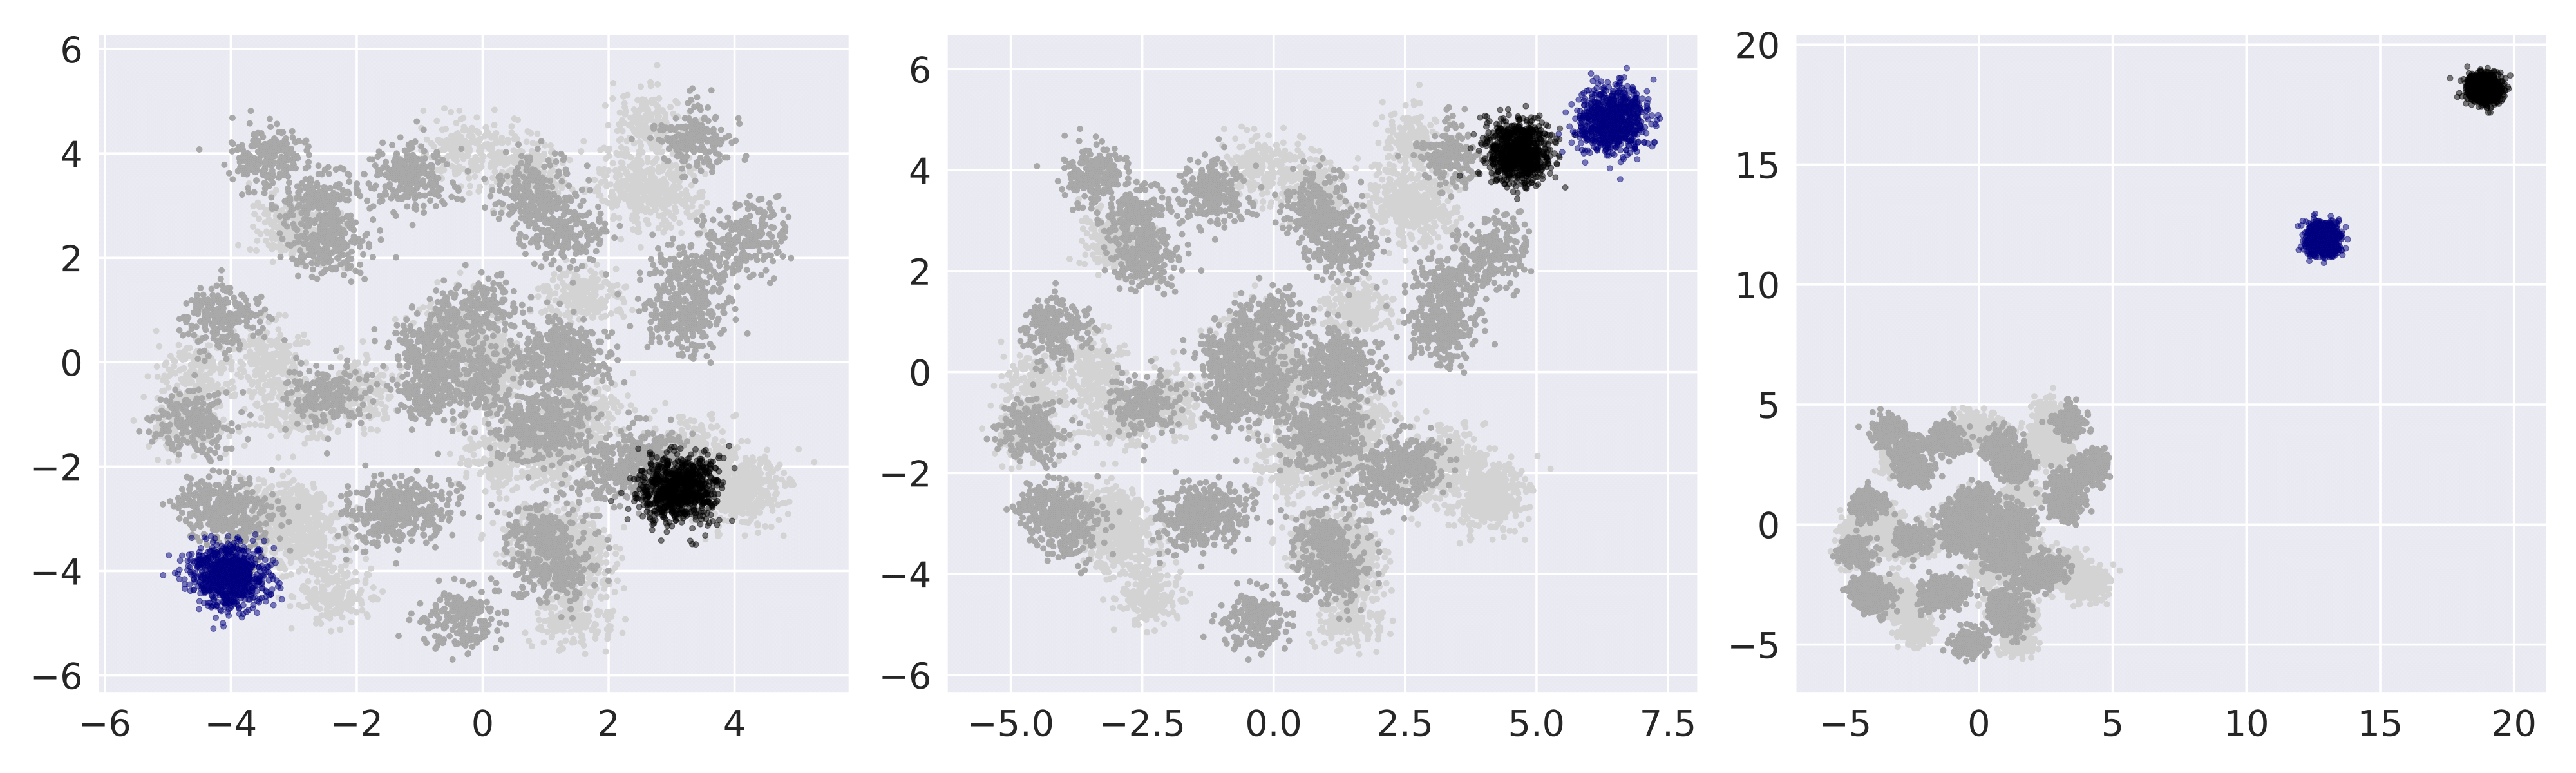
\includegraphics[ width=\linewidth]{images/chapter5/generalization_schemes.png}
\caption{Thirty mixtures drawn from the meta-distribution $\mathcal{M}$. We plot (in color) 3 unseen distributions whose parameters are drawn from (left) $U(-5, 5)$; (middle) $U(3,7)$; (right) $U(10, 20)$, the first two begin in and close to $\mathcal{M}$ whereas the last mixture is clearly outside of $\mathcal{M}$.}
\label{fig:mnist:gen}
\end{figure}

\section{Clustering Mixtures of Gaussians}
First, we present a simple clustering example to build intuition for meta-inference. Consider a standard VAE trained to capture a single mixture of two Gaussian (MoG) distributions $p_{\textup{data}}(x)$. Each component has isotropic covariance of $0.1$ and mean drawn from the uniform distribution, $U(-5, 5)$. The two components are mixed evenly and assigned a label of 0 or 1.
Then, inference $q_\phi(z|x)$ with  $z \in \{0, 1\}$ as a 1-D binary latent variable amounts to predicting which component $x$ belongs to, of which the true cluster label is recoverable up to a permutation.
Figure~\ref{fig:mnist:gen} shows a visualization of 30 mixtures from the meta-distribution. 

Given that an inference model $q_\phi(z|x)$ of a VAE can learn to cluster data from a \emph{specific} MoG, a meta-inference model $g_\phi(p_{\textup{data}_i},x)$ should correspond to \textit{a general-purpose clustering algorithm} that can separate out the components of any related, but previously  unseen mixture distribution $p_{\textup{data}_i}$. 
Concretely, we let each distribution $p_{\textup{data}_i} \sim p_\mathcal{M}$ be a MoG
% , where we represent each $p_{\textup{data}_i}(x)$ as a data set of samples $\mathcal{D}_i = \{x_1, ..., x_N\} \sim p_{\textup{data}_i}(x)$. 
% Thus, the meta-inference model $\hat{g}_\phi(\mathcal{D}_i, x)$ takes as input the data set as well as an observation $x \sim  p_{\textup{data}_i}(x)$.
and train a MetaVAE amortized over $N$ mixtures
% distributions from $p_{\mathcal{M}}$ 
to assess how well it can predict $z \in \{0,1\}$ for a given $x$ for an \emph{unseen test distribution}. 
% Like the VAE, meta-inference is equivalent to prediction. 
We measure this clustering accuracy on 1000 unseen but related MoGs 
sampled from the same meta-train distribution.
%with newly sampled component means from $U(-5, 5)$. 
While the VAE has a clustering error of $27.9$\% due to cases where there is extreme overlap in mixture components,
% \s{error seems way too high? might want to explain this}
the MetaVAE has an error of 9.9\% when $N = 50$. 
% \cc{Latter part of the sentence doesn't add much... 50 seems actually quite dense in the 2d space of possible configurations of means} 
% which is encouraging since 50 is a small number of the infinite possible mixture distributions in $\mathcal{M}$.
Moreover, larger $N$ improved the model's performance ($21.2$\% error with $N=10$ and $15.8$\% error with $N=20$) as expected. 
% which is sensible as the model sees more of the meta-distribution. 

\section{Inference for Classical Mechanics}

For a second demonstration, we consider an introductory problem in classical mechanics: objects sliding down inclined planes. Here, we are given a physics simulator that models a box that faces friction with the plane. 
% with the surface of a slope the box is set on. 
Each time the simulator runs, we see a new box with a different friction coefficient. The simulator then records the time it takes for the box to descend to the bottom of the plane. 
% Finally, say not all simulators are created equal, 
Each simulator has a different incline plane of length $L$ and incline angle $A$, and our task is to infer the coefficient of friction ($z$) from the observed descent time $(x)$ given a new simulator. 
\begin{figure}[h!]
\centering     %%% not \center
\includegraphics[width=0.9\linewidth]{images/chapter5/planes.pdf}
% \subfigure[]{\includegraphics[width=0.14\linewidth]{figures/physics/plane1.pdf}}
% \subfigure[]
% {\includegraphics[width=0.10\linewidth]{figures/physics/plane2.pdf}}
% \subfigure[]
% {\includegraphics[width=0.74\linewidth]{figures/physics/compiled.pdf}}
\caption{(a,b) Examples of planes with two lengths and angles. Mean squared error (MSE) between true and inferred friction for 304 simulators (lighter is better) using (c) MetaVAE and (d) VAE.}
\label{fig:physics}
\end{figure}
Building on \cite{le2016inference}, we tackle this problem with ``meta-compiled inference" and optimize: 
% \cc{good to write the \(p_{\theta^*_i}\) expectation in the \(\cdot \sim \cdot \) form for consistency}
% , where we optimize the following (see Appendix for derivation):
\begin{equation}
    \mathcal{L}_{\phi} = \mathbf{E}_{p_{\theta_i^*} \sim p_{\mathcal{M}}} \mathbf{E}_{x \sim p_{\theta_i^*}(x)}\left[-g_\phi(z| p_{\theta_i^*}, x) \right]
\end{equation}
The meta-distribution $\mathcal{M}$ represents all possible simulators of planes with $L \in [1,20]$ and $A \in [5,85]$ degrees, and $p_{\theta_i^*}(x, z)$ represents a fixed simulator. The marginal distribution, $p_{\theta_i^*}(x)$ is obtained by repeatedly simulating to build a data set $\mathcal{D}_i = \{ x \}$. Thus the empirical meta-inference model $\hat{g}_\phi(\mathcal{D}_i, x)$ takes the data set and the output of a single simulation $x$ as input. We amortize over 25 simulators with $L \in \{2,4,6,8,10\}$ and $A \in \{20,30,40,50,60\}$, and model $z$ as a continuous 1-D random variable (interpreted as friction). After training the MetaVAE, we measure the mean squared error between the true and inferred friction for unseen simulators from $\mathcal{M}$.
% We train a MetaVAE. Then, we freeze the encoder and docompiled inference for 300 generative models specified using lengths from 1 to 20 and angles from 5 to 80. We measure the MSE between inferred and true friction.
Despite seeing only 25 out of 304 simulators, the MetaVAE transfers well: we get less than 0.001 MSE for $A \in [20,70]$ and $L \in [2,20]$. A standard VAE trained on a single simulator ($L=10$, $A=45$) exhibits both much worse generalization performance and greater error overall (notice the scale in the legends). 
% \js{not sure if this is a fair comparison against VAE; what is specific here about the need of using VAE instead of a general probabilistic model to predict the coefficient?}

\section{Learning Distribution Statistics}
Next, we explore whether the MetaVAE is capable of "meta-learning" the concept of a sufficient statistic for exponential families~\cite{wainwright2008graphical}.
%random samples from several families of distributions. 
%In particular, we focus on the exponential family, as it is well known to encompass many common probability distributions \cite{wainwright2008graphical}.
% All distributions in the exponential family can be represented by a parameter (e.g. probability of success for a Bernoulli distribution). 
Given a set of random samples, a sufficient statistic is a function that maps this set to a vector in $\mathbb{R}^d$. For the exponential families, where each family member has the form \(p(x) \propto \exp (\theta \cdot \phi(x))\) for some parameter \(\theta\), this vector can be used to estimate the parameters of the distribution.
% For example, the sufficient statistic for realizations from a Gaussian random variable with fixed mean would return $x^2$, which is closely related to variance. 
In other words, the random samples (dataset) can be fully summarized by
% by the scalar value, and consequently 
the sufficient statistic, without any loss of information. 
% But more importantly, a data set of samples from one of these random vectors can be summarized by their sufficient statistics without any loss of information. 
% For example, the sample mean fully describes realizations of a Gaussian random variable with fixed variance. 
Now consider a \textit{vector} of random variables $(x_1, \cdots, x_k)$, each distributed i.i.d from the same distribution with sufficient statistic $\phi(x_i)$. 
%For exponential families, the sufficient statistic of the random vector
%from realizations of the random vector 
%is the sum $\sum_{i=1}^k \phi(x_i)$.
For exponential families, the sum $\sum_{i=1}^k \phi(x_i)$
is a sufficient statistic for the random vector. 
%from realizations of the random vector 
%of the scalar outputs of the sufficient statistic on realizations of each random variable in the vector 
%\mike{@stefano, is this true for Gaussian RVec?}
%. 
%As an example, a function of the sum of the number of successes given observations of a Bernoulli random vector is a sufficient statistic. 
As an example, the number of successes is a sufficient statistic for a vector of i.i.d. Bernoulli, and the sample mean and variance are for a vector of Gaussians. 
With this intuition, we ask the following: having seen many realizations of random vectors from different exponential family distributions, can we learn a sufficient statistic for %realizations of 
a new random vector that will be sufficient for estimating the parameters of its unseen, underlying distribution?
% sufficient statistic for realizations of a new random vector from an unseen distribution?
We aim to use the MetaVAE's meta-inference network to learn this mapping.
% to (meta) learn sufficient statistics -- that is, the MetaVAE should learn 
% to map a (sufficiently large) number of observations of random vectors distributed according to an exponential family to the sufficient statistic. 
%Precisely, if we fix the marginal distribution, then the meta inference model $g_\phi(\cdot, x)$, now a function of only $x$, is optimized to approximate the sufficient statistic where $x$ is a vector of random variables. We represent the marginal as a set of vectors of random variables, $\{x'\}$, each vector being distributed as $x$ is. Refer to the appendix for more exposition and details.
More precisely, the meta inference model $g_\phi(p_{\textup{data}_i},x)$ should act (as a function of $x$) as a sufficient statistic for an unseen distribution $p_{\textup{data}_i}$. 

\paragraph{Data and Model Setup}
We use 
% \cc{Only distributions named after people should be capitalised}
Gaussian (fixed variance), log-normal (fixed variance), exponential, symmetric beta, Laplace (fixed location), and Weibull (fixed scale) 
%random variables 
as exponential families. We then construct a set $\mathcal{M}_{\mathcal{I}}$ of 20-D 
vectors of random variables where each component is  i.i.d. distributed according to the same distribution. 
By construction, a random variable in this set will have only one free parameter, which can be found using the statistic learned by the meta-inference network.
We further restrict $\mathcal{M}_{\mathcal{I}}$ by bounding the free parameter to be within a range (e.g. Gaussians with mean between -5 and 5). 
After training, we measure how well we can infer the distributional parameters using the meta-inference model as a learned statistic for observations from unseen distributions. We compute the mean squared error (MSE) between the inferred and true parameters. 
% We refer the reader to the appendix for more details.

\begin{figure}
\centering     %%% not \center
\begin{subfigure}[b]{0.49\linewidth}
    \includegraphics[width=\linewidth]{images/chapter5/gaussian_only_test_set_mu.png}
\end{subfigure}
\begin{subfigure}[b]{0.49\linewidth}
    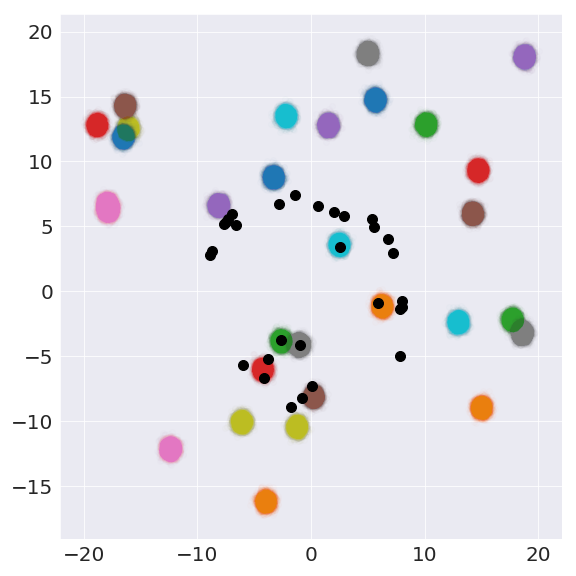
\includegraphics[width=\linewidth]{images/chapter5/gaussian_only_out_of_sample_set_mu.png}
\end{subfigure}
\begin{subfigure}[b]{0.49\linewidth}
    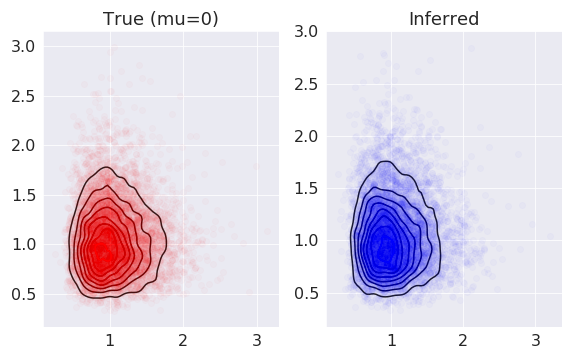
\includegraphics[width=\linewidth]{images/chapter5/lognormal_exapmle_good.png}
    \caption{Log Normal}
\end{subfigure}
\begin{subfigure}[b]{0.49\linewidth}
    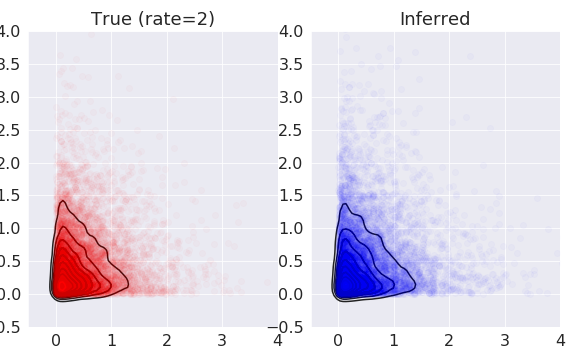
\includegraphics[width=\linewidth]{images/chapter5/exponential_exapmle_good.png}
    \caption{Exponential}
\end{subfigure}
\caption{Colored circles represent 30 different $p_{\textup{data}_i} \sim p_{\mathcal{M}}$; black dots represent the inferred Gaussian means from the meta-inference model. (a) Test Gaussian distributions within $\mathcal{M}$; (b) Test distributions outside of $\mathcal{M}$. (c,d) Samples from the an unseen Log Normal or Exponential distribution $p_{\textup{data}_i} \in p_{\mathcal{M}}$ (red) and the true corresponding distribution defined by the inferred statistic (blue).}
\label{fig:gaussian_plot}
\end{figure}

\paragraph{Single Exponential Family}
Each $p_{\textup{data}_i}(x) \in \mathcal{M}$ is Gaussian with a mean sampled from $U(-5, 5)$.  At test time, we measure inference quality on (1) new random vectors from $\mathcal{M}$ whose entries are distributed as Gaussians with unseen means sampled from $U(-5, 5)$, and (2) a larger meta-distribution by sampling means from $U(-20, 20)$. We find the MetaVAE successfully learns the mean of the underlying Gaussians. Interestingly, in Figure~\ref{fig:gaussian_plot}(a), we find that the inference quality only decays near the boundary of the meta-distribution.
% For example, see the purple Gaussian near $(5, 5)$. In Figure~\ref{fig:gaussian_plot}(b), we also find that the meta-inference model is almost bounded within the $[5,5]$ square centered at the origin as it is unable to do inference for distributions outside of $\mathcal{M}$.
% \kristy{took out the sentence below, feel free to add back in}
% Finally, Figure~\ref{fig:gaussian_plot}(c) plots the MSE of the inferred statistic, enumerating over Gaussian distributions with means from $-10$ to $10$. 
We compare the MetaVAE to a VAE trained on one Gaussian distribution and find that doubly-amortizing increases the inference quality dramatically.
% \vspace{-1em}
%\paragraph{Log Normal and Exponential Marginals. } 
Then we move to two new exponential families: we similarly construct 30 log-normal random vectors with means from $U(-2, 2)$ and 30 Exponential random vectors with rates sampled from $U(0, 3)$. Like above, Figure~\ref{fig:explognorm_plot} shows good performance of meta-inference over $\mathcal{M}$ in each case.
\begin{figure}
\centering     %%% not \center
\begin{subfigure}[b]{0.34\linewidth}
    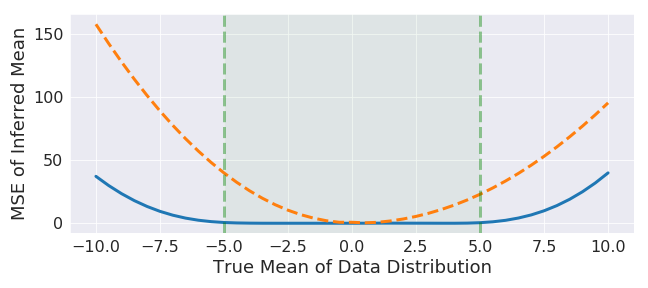
\includegraphics[width=\linewidth]{images/chapter5/gaussian_timeseries_plot.pdf}
    \caption{Gaussian}
\end{subfigure}
\begin{subfigure}[b]{0.31\linewidth}
    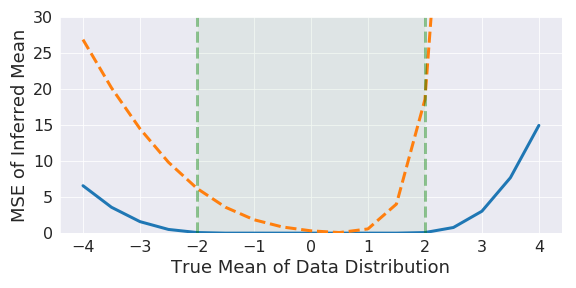
\includegraphics[width=\linewidth]{images/chapter5/lognormal_timeseries_plot.pdf}
    \caption{Log-Normal}
\end{subfigure}
\begin{subfigure}[b]{0.31\linewidth}
    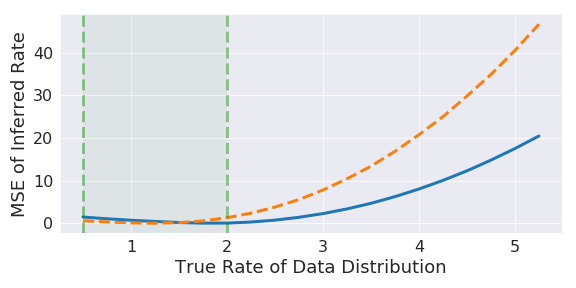
\includegraphics[width=\linewidth]{images/chapter5/exponential_timeseries_plot.pdf}
    \caption{Exponential}
\end{subfigure}
\caption{(a) Mean squared error (MSE) between the true and inferred mean as the true mean of $p_{\textup{data}_i}$ spans $[-10, 10]$. The green region shows the  meta-distribution. 
% \cc{Say orange (dashed), blue (solid) etc}
The orange (dashed) line shows a singly-amortized VAE trained on a single $p_{\textup{data}_i}(x)$ with mean $[-1.2, 1.1]$ (randomly chosen) and the blue (solid) line shows the MetaVAE. 
% \cc{There is no d here} 
(b,c) show the MSE between the true and inferred parameters. The orange line is a singly-amortized VAE trained on a  randomly chosen distribution ($[-0.5, 1.8]$ for log-normal; $[1.4, 2.8]$ for exponential).}
\label{fig:explognorm_plot}
\end{figure}
% \noindent
% \vspace{-1em}
\paragraph{Many Exponential Families} 
Finally, we amortize over many types of distributional families simultaneously: we construct sets of 30 Gaussian, 30 log-normal, and 30 exponential random vectors (same bounds as above) to train a MetaVAE. This setup raises an interesting question: can we do inference for new random vectors comprised of \textit{unseen members of the exponential family} (e.g. Weibull)? 

We compare the performance a MetaVAE amortized over the 90 random vectors to 3 different (baseline) MetaVAEs, each of which is amortized over only 30 random vectors from one family (e.g. Gaussian). Below, Figure~\ref{fig:expfam_plot}(a-c) plot the MSE of inferred and true parameters for Gaussian, log-normal, and exponential (all of which are in $\mathcal{M}$). Due to the double-amortization gap, the best performing model is the MetaVAE amortized on random vectors only from that family. However, the 90-amortized MetaVAE only performs slightly worse, beating the remaining two baselines dramatically. Next, Figure~\ref{fig:expfam_plot}(d-f) show MSEs for three distributions not in $\mathcal{M}$: Weibull, Laplace, and Beta. The 90-amortized MetaVAE consistently outperforms all baselines. 
% This hints that amortizing inference over the exponential families together enables the model to learn more robust representations.

\begin{figure}[h]
\centering     %%% not \center
\begin{subfigure}[b]{0.9\linewidth}
    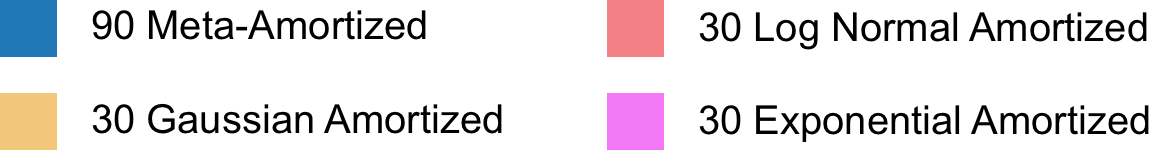
\includegraphics[width=\linewidth]{images/chapter5/legend.pdf}
\end{subfigure}
\begin{subfigure}[b]{0.32\linewidth}
    \includegraphics[width=\linewidth]{images/chapter5/mixed_gaussian_timeseries_plot.pdf}
    \caption{Gaussian}
\end{subfigure}
\begin{subfigure}[b]{0.32\linewidth}
    \includegraphics[width=\linewidth]{images/chapter5/mixed_lognormal_timeseries_plot.pdf}
    \caption{Log Normal}
\end{subfigure}
\begin{subfigure}[b]{0.32\linewidth}
    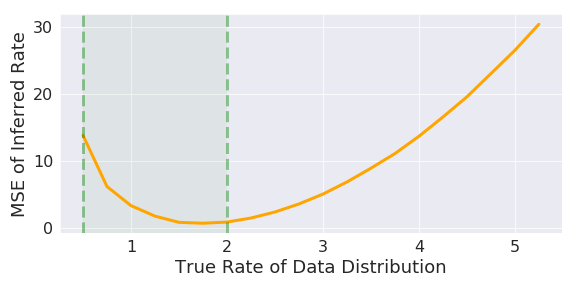
\includegraphics[width=\linewidth]{images/chapter5/mixed_exponential_timeseries_plot.pdf}
    \caption{Exponential}
\end{subfigure}
\begin{subfigure}[b]{0.32\linewidth}
    \includegraphics[width=\linewidth]{images/chapter5/beta.pdf}
    \caption{Beta($\alpha$, $\alpha$)}
\end{subfigure}
\begin{subfigure}[b]{0.32\linewidth}
    \includegraphics[width=\linewidth]{images/chapter5/weibull.pdf}
    \caption{Weibull(scale=1)}
\end{subfigure}
\begin{subfigure}[b]{0.32\linewidth}
    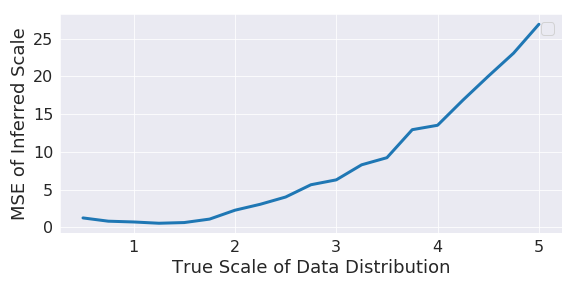
\includegraphics[width=\linewidth]{images/chapter5/laplace_scale.pdf}
    \caption{Laplace(loc=0)}
\end{subfigure}
\caption{Comparison of a MetaVAE amortized over three members of the exponential family to MetaVAEs amortized over only a single member. Each subplot shows an unseen distribution from either the meta-distribution (b,c,d) or another exponential family (e,f,g).}
\label{fig:expfam_plot}
\end{figure}

\section{Transformation-Invariance Experiments}
Imagine designing a scene understanding algorithm for a self-driving car. The video datasets used to train deep learning agents are typically collected in isolated settings, such as in large cities during favorable weather conditions.
% such as only at morning or night, or only in large cities. 
However, an agent deployed in the real world may face a variety of new settings such as paved roads in poorly-lit suburban areas.
% when deploying an algorithm in the real world, it may face all kinds of settings we have not seen beofre such as dusk or roads in small suburban communities. 
In such cases, we would hope the agent could abstract away unnecessary sources of variation, such as different lighting conditions, and act upon more salient characteristics in the scene (e.g. pedestrians) that it has seen previously during training. 
Inference in this scenario would mean learning representations that are "transferable," or invariant to nuisance transformations such as time of day.
% If we consider inference in this scenario, for a latent representation to be ``transferable", it must be invariant to different transformations that we deem irrelevant, such as time of day. 
We take a step towards this goal as 
% One of the benefits of meta-inference is learning a more transferable representation that can capture features representative all amortized distributions. To highlight this,
we study the MetaVAE for image distributions with explicit transformations, such as rotations or lighting. 
 
% \vspace{-1em}
We study MNIST \cite{lecun1998mnist} and NORB \cite{lecun2004learning}, where we amortize over three axes of variation each (e.g. a range of camera angles or background lighting). Further, we vary how different variations are split into meta-training and meta-test sets, summarized in Fig.~\ref{fig:splits}(a-c). For instance, we may train the MetaVAE only on images with bright backgrounds and evaluate on darker images. We consider three meta-splits: \textit{interleaved}, where every other value in the range of possible transformations is selected; \textit{sparse}, where half the number of values are chosen as in interleaved; \textit{contiguous}, where we split the range in two ``contiguous" halves and train only over the first half. Each meta-split is a different measure of transfer-ability. 
% We defer further details regarding dataset construction to the next section.
% \s{i feel that a digram showing the various meta datasets, meta test, etc pictorially would be very helpful (to put in appendix). showing digits grouped by rotation (say) and how they are used for train and test, labeling the $D_i$, $g$, etc}
% mw: i made a diagram

 \begin{figure}
    \centering
    \begin{subfigure}[b]{0.21\linewidth}
        \includegraphics[width=\linewidth]{images/chapter5/split_interleaved.png}
        \caption{Interleaved}
    \end{subfigure}
    \hspace{1em}
    \begin{subfigure}[b]{0.21\linewidth}
        \includegraphics[width=\linewidth]{images/chapter5/split_sparse.png}
        \caption{Sparse}
    \end{subfigure}
    \hspace{1em}
    \begin{subfigure}[b]{0.21\linewidth}
        \includegraphics[width=\linewidth]{images/chapter5/split_disjoint.png}
        \caption{Contiguous}
    \end{subfigure}
    \begin{subfigure}[b]{0.8\linewidth}
        \includegraphics[width=\linewidth]{images/chapter5/model_image.pdf}
        \caption{Meta-Inference Pipeline}
    \end{subfigure}
    \caption{(a-c) Three ways of defining the meta-training and meta-test splits; (b,c) pose a more difficult generalization challenge. (d) Overview of the doubly-amortized inference procedure. The meta-training set is used to train the MetaVAE (the test portion is to used to choose best parameters). The meta-test set is for evaluating the learned features, where the training portion is used to fit a linear classifier and the test portion is used to compute accuracy.}
    \label{fig:splits}
\end{figure}
 

% \vspace{-1em}
\paragraph{Evaluation Metric} We evaluate the latent representations on a downstream classification task. Having trained the empirical meta-inference model $\hat{g}_\phi(\mathcal{D}, x)$ using the meta-train set, we then embed observations from a distribution in the meta-test set. Each time we ``embed'' a test observation $x$, we feed in a data set $\mathcal{D}$ of samples \emph{from the meta-test set}. This way we construct a data set of latent features.

This feature set is split into a training and test subset. For both MNIST and NORB, each image has a corresponding label (e.g. digit or object class). 
% that we so far have not used. 
Using the training portion (darker red in Fig.~\ref{fig:splits}d) , we fit a logistic regression classifier on the representations to predict the labels and compute accuracy on the test subset (lighter red in Fig.~\ref{fig:splits}d). 
Critically, logistic regression seeks the best linear split between classes in the latent space. For it to achieve good accuracy, such a linear division must already exist.
% meaning that the information must be contained explicitly in the features. 
Thus, we treat a higher classification accuracy as a more transferable, invariant representation, as in \cite{berthelot2018understanding}.

\paragraph{Baselines} We compare the performance of MetaVAE against two baselines: the Neural Statistician (NS), a hierarchical VAE which models sets of observations with a global latent variable; and the Variational HomoEncoder (VHE), a more computationally-efficient variant of  NS. To ensure a fair comparison, we use the same hyperparameters and architectures across all models.

\begin{figure}
    \centering
    \includegraphics[width=0.9\textwidth]{images/chapter5/datasets_subset.png}
    \caption{Examples of interpolating across three transformations each for MNIST and Small NORB. Notice that for NORB (unlike MNIST), other transformations are not held constant as we vary an individual axis.}
    \label{fig:datasets}
\end{figure}

\paragraph{Transformed MNIST}

We artificially impose three axes of variations on MNIST digits. We transform each image with 18 \textit{rotations} (-180 to 180 by 20 degrees), 15 \textit{scales} (50\% to 200\% original size by 10\%), and  18 \textit{skews} (-180 to 180 by 20 degrees). 
% \cc{Is it worth disucssing the fact that flipping a 9 by 180 deg changes the label?}
See Fig.~\ref{fig:datasets}(a-c) for an example for a single digit. For each axes of variation, the other two are held constant e.g. skew and size are constant when varying rotation. 

% \vspace{-1em}
We find consistent evidence that MetaVAE features outperform both VHE and NS features across all settings, often by a significant margin. In particular, VHE and NS have decaying performance as scale increases to 2.0. Similarly, for extreme shear values near -80 and 80 degrees where the image is nearly flat (see Fig.~\ref{fig:datasets}c), VHE and NS again suffer greatly in performance.
% , understandably as these are aggressive shearing values. 
However, MetaVAE features transfer better: we do not notice a drop in accuracy as scale increases and the effect of significant shearing is more gradual. 
This suggests that MetaVAE has learned some invariances to transformations that NS and VHE lack.

\begin{figure}
    \centering
    \includegraphics[width=0.9\textwidth]{images/chapter5/results.pdf}
    \caption{Classification Accuracy on Transformed MNIST and Small NORB for three different splits: interleaved, sparse, and contiguous. Each subfigure shows the prediction accuracy on the test set of held out transformations --- gaps represent the values used in training the amortized generative model. We compare the performance of MetaVAE (black), the homoencoder (blue) and the statistician (red) and find appealing results for our proposed model.} 
    % \cc{I don't understand how it's possible to get over 80\% accuracy on 180 deg rotated MNIST if two of the classes (6 and 9) swap labels under transformation}}
    \label{fig:invariance:results}
\end{figure}

\paragraph{Small NORB}

The NORB dataset contains grayscale images of real world toys belonging to five classes: animals, humans, airplanes, trucks, and cars. The objects were imaged under 6 \textit{lighting} conditions, 9 \textit{elevations} (30 to 70 degrees every 5 degrees), and 18 \textit{azimuths} (0 to 340 every 20 degrees). Unlike the MNIST dataset, extraneous transformations are \textit{not} held constant as one transformation is varied. For example, as Fig.~\ref{fig:datasets}(f) shows, the azimuth and elevation (randomly) change as we vary lighting. This design, while more difficult to amortize, is more realistic in real world datasets where it is too expensive to collect data holding all other variables constant.

The MetaVAE representations outperform those of VHE and NS by 10 to 35\% accuracy. Overall, we notice accuracies are much lower in NORB than in MNIST, which is likely due to the complexity of learning real world image distributions and randomness from extraneous transformations. 
% Unlike MNIST, we no longer see VHE outperforming NS --- often the two accuracies are close to identical. 
We note that the strong performance of the MetaVAE despite varying transformations is promising support for our approach to meta-amortization, suggesting that the MetaVAE is able to ignore irrelevant signals while capturing the principal axes of variation.

\paragraph{Analysis}
We aim to quantitatively measure the intuition that amortizing over a family of transformations should yield representations that are invariant to that transformation.
% that transfer better to related perturbations across that axis of variation. 
% One of doing this is to we compare the effects of varying transformations on the learned representations.
% Next, we aim to quantitatively measure the effect of varying transformations on the learned representations.
% the intuition that ``varying transformations are being merged together." Specifically, we want to compare the learned embeddings as the transformation changes. 
For example, how much does the representation change as we alter the rotation in MNIST from -180 to 180, or interpolate the background from dark to light in NORB? 
To investigate, we use a MetaVAE amortized over a family of transformations (e.g. interleaved rotations) and compare the average
% \footnote{We average across a family of transformations (e.g. rotations of -180 to 180 by 20 degrees) and over images in the test set.} 
L$_2$ distance between the learned representation of a base (default) image and those of every rotated image. As a baseline, we compare this distance to the average L$_2$ distance of a separate family of transformations (e.g. scale) that this MetaVAE was not amortized over (e.g. having only seen different rotations during training). Table~\ref{table:distance} shows the distances for MNIST and NORB. Consistently, the lowest distances belong to the class of transformations that the MetaVAE was amortized over, which supports the intuition about learning invariances.

% \kristy{can't use tiny either :(}
\begin{table}[h]
\centering
% \tiny  
\begin{tabular}{r|c|c|c}
\toprule
Model Dataset & Rotation & Scale & Skew \\
\midrule
Rotated MNIST & $\mathbf{1.65}$ & $4.44$ & $4.09$ \\ 
Scaled MNIST &  $5.44$ & $\mathbf{2.16}$ & $4.92$ \\  
Skewed MNIST & $3.79$ & $4.89$ & $\mathbf{1.47}$ \\   
\toprule
Model Dataset & Elevation & Azimuth & Lighting \\
\midrule
NORB Elevation & $\mathbf{0.39}$ & $1.16$ & $1.27$ \\ 
NORB Azimuth &  $1.42$ & $\mathbf{0.44}$ & $1.26$ \\  
NORB Lighting & $1.69$ & $1.27$ & $\mathbf{0.26}$ \\
\bottomrule
\end{tabular}
\caption{L$_2$ distances between MetaVAE representations. Each row indicates the datasets  used for training; each column indicates the datasets used to compute representations post-training.}
\label{table:distance}
\end{table}

\section{Related work}
\paragraph{Rapid Adaptation through Meta-Learning.} Among the rich body of work on meta-learning \cite{vinyals2016matching,snell2017prototypical,gordon2018decision}, a common goal is to train models such that they will rapidly adapt to new, unseen classification tasks. Although the Neural Process (NP) \cite{garnelo2018neural,kim2019attentive} is similar to our work in that it derives predictions for new targets by conditioning the encoder network on a relevant \textit{context set}, it models uncertainty over a distribution of \textit{functions}.
Another line of research formulates proper initialization as the workhorse of successful meta-learning \cite{finn2017model,grant2018recasting}. Our meta-amortized inference procedure can be thought of as learning a good initialization for an inference model on a new target distribution. However, these approaches are not directly comparable because of their supervised nature. 

% \vspace{-1em}
\paragraph{Few-shot Generative Modeling.} This branch of research aims to train generative models such that they will generalize to unseen distributions at test time given only a few examples. The focus has been on few-shot density estimation, with approaches ranging from the use of
% attention \cite{rezende2016one}, 
conditioning \cite{bartunov2016fast} to nested optimization \cite{reed2017few}. Meta-inference however is not few-shot, and instead aims to learn transferable \textit{representations} for downstream tasks rather than density estimation alone.
% Although meta-inference aims to transfer to new distributions, it is not few-shot and instead prioritizes learning representations for downstream tasks rather than density estimation alone.
%that will generalize well to downstream tasks such as classification.

% \mike{it might be useful to write the losses for NS and VHE? that way we can accent the global variable more -- hard to understand what it is atm. also since we pushed all summary network stuff to the appendix, may not be worth mentioning here}
The most relevant prior works include the Neural Statistician \cite{edwards2016towards} (NS) and the Variational Homoencoder \cite{hewitt2018variational} (VHE), two very similar models that study inference over sets of observations. The VHE optimizes the following objective, 
% \cc{Can put \(x,\mathcal{D} \sim p_\mathcal{D}\) instead of two lines?}
% mw: we can take this out if we want it but i think its good to be explicit
\begin{equation}
    \mathbf{E}_{x,\mathcal{D} \sim p_{\textup{data}}}[\mathbf{E}_{z \sim q_\phi(c|\mathcal{D})}[\log p_\theta(x|c)] - \frac{1}{N}\textup{KL}(q_\phi(c|\mathcal{D}), p(c))]
    \label{eqn:homoencoder}
\end{equation}
where $\mathcal{D} = \{x_1, ..., x_N\}$ is a set of $N$ samples and $c$ is a global latent variable. 
% \cc{What is \(c\)?If it's just the same as \(z\), should just put it in as \(z\)}
We note that if we view $\mathcal{D}$ as an approximation for a marginal distribution, then NS and VHE also serve as baselines that can perform doubly-amortized inference. Like our proposed inference model $\hat{g}_\phi(\mathcal{D}, x)$, the distribution $q(c|\mathcal{D})$ in Equation~\ref{eqn:homoencoder} ingests a data set.
% cast the inference problem as learning a distribution over a \textit{set} of related distributions. 
However, both the VHE and NS utilize a global variable $c$ (isotropic Gaussian). 
% \cc{Ok, \(c\) is here. If possible, maybe try to rewrite this so the \(c\) isn't dangling for too long}
We believe this constraint is \textit{overly restrictive} in settings which require transferring to a diverse set of distributions, hurting generalization performance. Instead, the MetaVAE does not impose a distributional assumption, and we find that this non-parametric approach yields consistently better performance. 

\section{Conclusion}
In summary, we considered constructing an algorithm that can do inference for a  \textit{family} of probabilistic models. We introduced a meta-amortized inference paradigm and a new generative model, the MetaVAE. 
Through experiments on MNIST and Small NORB, we showed that the MetaVAE learned transferable representations that generalize well across similar data distributions in downstream tasks. 
% Through experiments on MNIST and Small NORB, we found good classification performance from the learned representations that suggests a notion of transformation invariance. 
Future work could consider new applications of meta-inference in video prediction \cite{ramanathan2015learning}.